\subsection{1018MS Corrosion Parameters from Anodic/Cathodic Sweeps}

	\begin{figure}[h!]
		\centering
		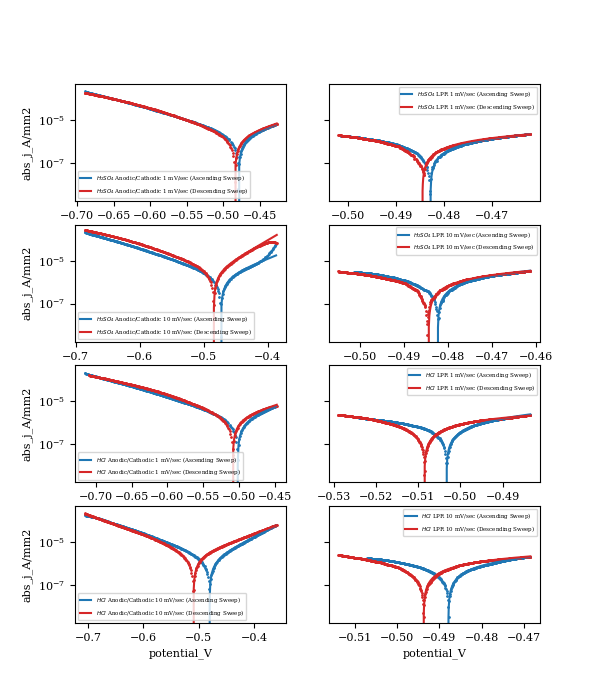
\includegraphics[width=5.0in]{resources/fig_2b.png}
		\caption{Results of fitting Equation \ref{eqn:bv_tafel} to the eight 1018MS polarization sweeps.  The scales of the axes indicate little variation in the current densities and potentials relative to SCE among the sweeps, though the limited scope of the LPR sweeps produced a large variance in their calculated parameters.}
		\label{fig:anocat}
	\end{figure}

	\begin{table}[h!]
		\centering
		\begin{tabular}{lllrrrr}
\toprule
  &     &     &  $A_{\text{H}}$ (V) &  $A_{\text{Fe}}$ (V) &  $j_{\text{corr}}$ (A/mm$^2$) &  $\Delta \phi_{\text{corr}}$ (V) \\
Scan & Soln & Dir &                     &                      &                               &                                  \\
\midrule
0 & H$_2$SO$_4$ & Asc &          -8.778e-02 &            8.903e-02 &                     1.784e-06 &                       -4.794e-01 \\
  &     & Des &          -9.588e-02 &            8.833e-02 &                     1.888e-06 &                       -4.843e-01 \\
2 & H$_2$SO$_4$ & Asc &          -8.341e-02 &            8.519e-02 &                     1.663e-06 &                       -4.730e-01 \\
  &     & Des &          -5.730e-02 &            8.076e-02 &                     3.096e-06 &                       -4.842e-01 \\
4 & HCl & Asc &          -7.706e-02 &            8.553e-02 &                     1.277e-06 &                       -5.022e-01 \\
  &     & Des &          -9.978e-02 &            8.326e-02 &                     1.765e-06 &                       -5.090e-01 \\
6 & HCl & Asc &          -7.490e-02 &            9.225e-02 &                     1.469e-06 &                       -4.806e-01 \\
  &     & Des &          -1.035e-01 &            8.415e-02 &                     2.140e-06 &                       -5.097e-01 \\
\bottomrule
\end{tabular}

		\caption{Derived parameters for Equation \ref{eqn:bv_tafel} (Tafel slopes, corrosion currents, and corrosion potentials relative to SCE) for 1018MS anodic/cathodic sweeps.  See Appendix C for associated variances.}
		\label{table:anocat}
	\end{table}

All collected 1018MS polarization sweeps were fit to the form of Equation \ref{eqn:bv_tafel} using the Python package \textit{lmfit}.\cite{lmfit}  Since Equation 1 does not account for diffusion-limited behavior, each fitting was performed within a narrow data window of width 100 mV centered on the corrosion potential.  The quality of fits varied: while the parameters derived from the LPR scans possessed much smaller variances due to their greater data densities, the parameters derived from the Ano/Cat scans were far more consistent in terms of value.  The fitted parameters and variances from the designated Ano/Cat scans are presented in Table \ref{table:anocat}, while the according fits are plotted against the data in Figure \ref{fig:anocat}.  All fitted parameters for the eight 1018MS scans, as well as their variances, may be found in Appendix 3.

Using solely the data from the Ano/Cat scans (Scans 0, 2, 4, and 6), the average values of the Tafel slopes were found to be $A_{\text{H}} = -8.620$e-02 V and $A_{\text{Fe}} = 8.606$e-02 V; the similarity in the magnitude of these values supports the assumption that $\beta \approx 0.5$ in Equation \ref{eqn:bv_raw}.  The average corrosion potential was found to be $\Delta \phi_{\text{corr}} = -0.4903$ V vs. SCE, with the associated average corrosion rate being $j_{\text{corr}} = 1.88$e-6 A/mm$_2$.  The variances in the equilibrium parameters were much smaller than their respective values ($\sigma^2(j_{\text{corr}}) = 2.14$e-15 A/mm$^2$, $\sigma^2(\Delta \phi_{\text{corr}}) = 5.41$e-8 V), but the variances of the Tafel slopes were found to be uncharacteristically large ($\sigma^2(A_{\text{H}}) = 99.5$ V, $\sigma^2(A_{\text{Fe}}) = 159$ V).  Given the similarities of the actual fitted parameters, however, this was though to be an error in statistical estimation rather than an indicator of actual variance in the Tafel slopes.

It should be noted that, in this analysis, variances were propagated using:

	\begin{equation}
		f(a_1, a_2, ...) \rightarrow \sigma^2_f = \sum_i \left( \frac{\partial f}{\partial a_i} \right)^2 \sigma^2_{a_i}
		\label{eqn:se}
	\end{equation}

It should also be noted that hystersis was observed within these scans; the observed corrosion potentials on the downward half of the sweeps were consistently lower than those of the upward halves.  A discussion of this hystersis is reserved for the Discussion.

\subsection{1018MS Corrosion Parameters from LPR Sweeps}

	\begin{table}[h!]
		\centering
		\begin{tabular}{llllrrrr}
\toprule
  &     &           &     &  $j_{corr}$ (A/mm$^2$) &  $\Delta \phi_{corr}$ (V) &  $\sigma^2(j_{corr})$ &    n \\
Scan & Soln & Rate & Dir &                        &                           &                       &      \\
\midrule
1 & H$_2$SO$_4$ & 1 mV/sec & Asc &              1.342e-06 &                -4.830e-01 &             6.559e-16 &  338 \\
  &     &           & Des &              1.354e-06 &                -4.841e-01 &             3.434e-15 &  421 \\
3 & H$_2$SO$_4$ & 10 mV/sec & Asc &              2.058e-06 &                -4.822e-01 &             2.552e-15 &  342 \\
  &     &           & Des &              1.941e-06 &                -4.849e-01 &             1.070e-14 &  444 \\
5 & HCl & 1 mV/sec & Asc &              1.302e-06 &                -5.032e-01 &             4.275e-14 &  353 \\
  &     &           & Des &              1.335e-06 &                -5.085e-01 &             2.300e-14 &  442 \\
7 & HCl & 10 mV/sec & Asc &              1.265e-06 &                -4.879e-01 &             4.494e-15 &  342 \\
  &     &           & Des &              1.297e-06 &                -4.937e-01 &             2.720e-14 &  443 \\
\bottomrule
\end{tabular}

		\caption{Fitting parameters for Equation \ref{eqn:bv_lpr}, as calculated from the LPR scans for 1018MS.  The fitting package \textit{lmfit} was unable to estimate the variance for $\Delta \phi_{\text{corr}}$.}
		\label{table:lpr}
	\end{table}

	\begin{figure}[h!]
		\centering
		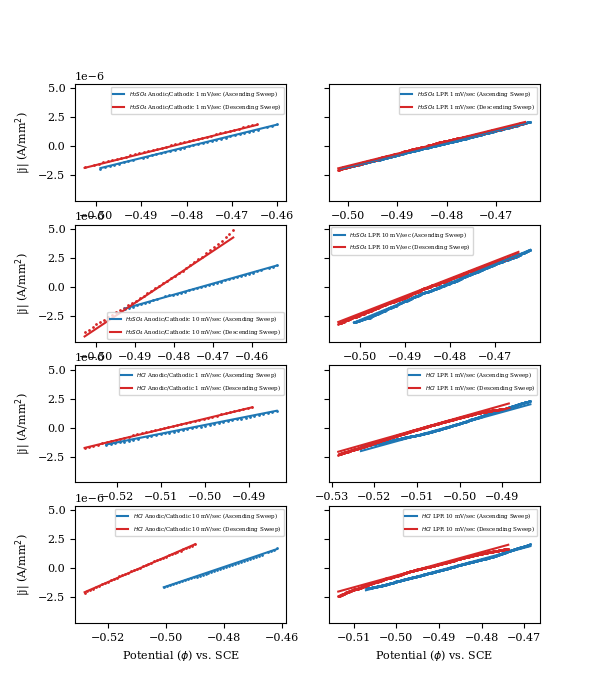
\includegraphics[width=5.0in]{resources/fig_2c.png}
		\caption{Linear fits in the low-overpotential regime for all eight 1018MS scans.}
		\label{fig:lpr}
	\end{figure}

Figure \ref{fig:lpr} shows the results of fitting Equation \ref{eqn:bv_lpr} to local linear regions of each of the 1018MS scans.  In the case of the dedicated LPR scans, this region comprised the entirity of the scans, while the Ano/Cat scans were trimmed to a window of $\Delta \phi_{\text{corr}} \pm 20$ mV in order to isolate a comparable region.  All 1018MS scans were found to possess linear behavior in the vicinity of $\Delta \phi_{\text{corr}}$, validating the LPR measurement approach.  The resulting parameters from the pre-designated LPR scans (Scans 1, 3, 5, and 7) are shown in Table \ref{table:lpr}, while the fitted parameters for all eight 1018MS scans are presented in Appendix 4.

Using these data, the average value for the corrosion current was found to be 1.49e-6 A/mm$^2$, with an associated variance of $\sigma^2(j_{\text{corr}}) = 1.79$e-15 A/mm$^2$.  The average value of the corrosion potential was found to be -4.910 V, though \textit{lmfit} estimated the variances of this parameter to be 0.

\subsection{Deconvolution of 304SS H$_2$SO$_4$ Polarization Sweep}

In order to analyze the 304SS polarization curves, the anodic and cathodic sweeps were concatenated.  In the case of the HCl curves, this did not require any modification; however, the cathodic H$_2$SO$_4$ curve exhibited a corrosion potential \textapprox 0.25 V higher than any other corrosion potential measured in this experiment.  This was assumed to be an experimental error; sa such, the data were shifted so that their corrosion potential aligned with that of the anodic curve.

For both the H$_2$SO$_4$ and HCl curves, the hydrogen reduction reaction was fit to the diffusion-limited model (Equation \ref{eqn:bv_w}) and subtracted out of the remaining data.  This was observed, however, to have little effect.  In particular, this deconvolution did not remove any other singularities or depressions in the curves, indicating that other reduction reactions were active within certain $\phi$-regimes.  The dominant reactions in portions of the H$_2$SO$_4$ curve were thus explained as follows:

\singlespacing
\begin{itemize}
	\item \textbf{$<$ \textapprox -0.4 V:} $2 \text{H}^+ + 2 e^- \rightarrow \text{H}_2$ (reduction of hydrogen ions to produce hydrogen gas, as evidenced by bubbling on the electrode surface)
	\item \textbf{\textapprox -0.4 V to \textapprox -0.3 V:} $\text{Fe} \rightarrow \text{Fe}^{2+} + 2 e^-$ (oxidation and dissolution of iron)
	\item\textbf{\textapprox -0.3 V to \textapprox 0 V:} $\text{Cr} \rightarrow \text{Cr}^{3+} + 3 e^-$ (passivation of electrode surface due to formation of Cr$_2$O$_3$, and intersection with an unknown reduction reaction, such as the reduction of acqueous Fe, Ni, or Cr)
	\item\textbf{\textapprox 0 V to \textapprox 0.9 V:} $\text{Cr} \rightarrow \text{Cr}^{3+} + 3 e^-$ (passivation of electrode surface due to formation of Cr$_2$O$_3$)
	\item\textbf{\textapprox 0.9 V to \textapprox 1.5 V:} $\text{Cr}^{3+} \rightarrow \text{Cr}^{6+} + 3 e^-$ (destruction of passivation layer to formation of aqueous HCrO$_4^-$, as evidenced by reddish-orange ion trails surrounding the electrode)
	\item \textbf{$>$ \textapprox 1.5 V:} $\text{H}_2\text{O} \rightarrow 2 \text{H}^+ + \frac{1}{2} \text{O}_2 + 2 e^-$ (breakdown of water, as evidenced by renewed bubbling on the electrode surface)
	\item \textbf{$<$ \textapprox 0.8 V on descending sweep:} $\text{Cr}^{6+} + 3 e^- \rightarrow \text{Cr}^{3+}$ (reduction of aqueous Cr to reconstruct the passivation layer)

\end{itemize}
\doublespacing

An attempt was then made to deconvolute the H$_2$SO$_4$ curve into contributions from its component reactions, as modelled using Equation \ref{eqn:bv_w}.  It was found, however, that Equation \ref{eqn:bv_w} could not fit the passivation region; furthermore, the presence of multiple singularities precluded a traditional stepwise model of the passivation potential, which would not be able to manifest the changes in concavity required to replicate these singularities.  Equation \ref{eqn:bv_w} was therefore modified by means of a changing resistivity:

	
	\begin{equation}
		\rho = \rho_{\text{lim}} + 
		\rho_{\text{pass}} \left[
			1 - \exp (- \alpha_{\text{pass}} \eta_{\text{pass}}^3) \right]
		\label{eqn:rho_jmak}
	\end{equation}

	\begin{table}[h!]
		\centering
		\begin{tabular}{lrrrr}
\toprule
{} &  $\phi_0$ (V) &  $j_0$ (A/mm$^2$) &    $A$ (V) &  $\rho_{\text{lim}}$ ($\Omega \cdot$mm) \\
Reaction                             &               &                   &            &                                         \\
\midrule
H$^+$ reduction                      &    -3.728e-01 &        -9.612e-08 & -1.138e-01 &                               1.587e+02 \\
Fe oxidation (passivation-limited)   &    -3.927e-01 &         7.891e-07 &  3.505e-03 &                               3.905e+04 \\
Cr$_2$O$_3$ barrier breakdown (asc)  &     9.688e-01 &         9.902e-07 &  3.701e-02 &                               1.968e+03 \\
H$_2$O breakdown (asc)               &     1.596e+00 &         1.065e-04 &  2.025e-01 &                              3.230e-312 \\
unknown reduction reaction           &     1.500e-01 &        -5.000e-11 & -3.289e-02 &                               2.000e+05 \\
Cr$_2$O$_3$ solution deposition      &     1.070e+00 &       -1.812e+169 & -9.784e-06 &                               4.502e+06 \\
Cr$_2$O$_3$ barrier breakdown (desc) &     9.814e-01 &         4.565e-07 &  5.713e-02 &                               1.324e+03 \\
H$_2$O breakdown (desc)              &     1.599e+00 &         1.016e-04 &  1.971e-01 &                               3.765e-06 \\
\bottomrule
\end{tabular}

		\begin{tabular}{lrrr}
\toprule
{} &  $\phi_{pass}$ (V) &  $\alpha_{pass}$ (V$^{-3}$) &  $\rho_{pass}$ ($\Omega \cdot$mm) \\
Reaction                             &                    &                             &                                   \\
\midrule
Fe oxidation (passivation-limited)   &         -3.530e-01 &                   4.814e+00 &                         6.966e+06 \\
Cr$_2$O$_3$ barrier breakdown (asc)  &          1.300e+00 &                   8.971e-03 &                         5.670e+07 \\
unknown reduction reaction           &         -3.000e-02 &                   1.000e+01 &                         1.000e+07 \\
Cr$_2$O$_3$ barrier breakdown (desc) &          1.239e+00 &                   7.470e-03 &                         2.868e+07 \\
\bottomrule
\end{tabular}

		\caption{Deconvolution parameters for Equation \ref{eqn:bv_w} from the combined anodic/cathodic H$_2$SO$_4$ polarization sweep.  Four fitting regions required the JMAK resisitity modification outlined in Equation \ref{eqn:rho_jmak}.}
		\label{table:h2so4_deconv}
	\end{table}

	\begin{figure}[h!]
		\centering
		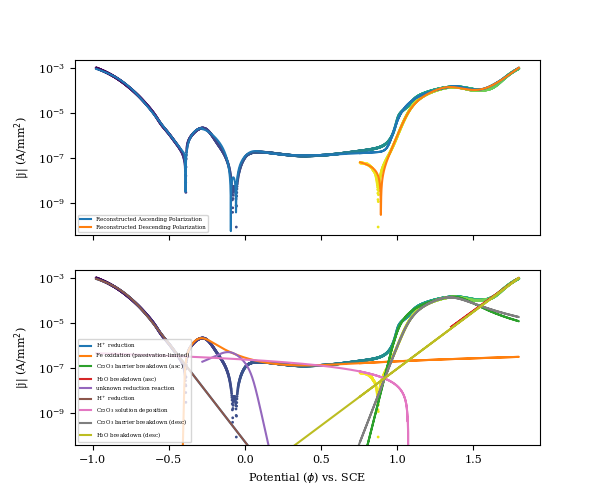
\includegraphics[width=5.0in]{resources/fig_2a1.png}
		\caption{Top: Fitted H$_2$SO$_4$ curves generated by deconvolution procedure.  Bottom: Individual reaction components fitted using Equations \ref{eqn:bv_w} and \ref{eqn:rho_jmak}.}
		\label{fig:h2so4_deconv}
	\end{figure}
This ``ansatz'' treats the passivation layer as an additional resistivity in series with that of the diffusion layer.  Its two-dimensional formation is modeled using Johnson-Mehl-Avrami-Kolmogorov kinetics.\cite{labguide_1}  Since the potential ramp rate is constant throughout the curve, time in the JMAK equation was replaced with the overpotential relative to the passivation potential ($\eta_{\text{pass}}$).  Such a form produces an s-curve that, while having no rigorous theoretical basis, nevertheless provides an improved fitting approximation of regions of the polarization curve.  The results of the deconvolution of the H$_2$SO$_4$ into individual reaction components are presented in Table \ref{table:h2so4_deconv}, while the resulting curves are presented in Figure \ref{fig:h2so4_deconv}.

From this analysis, the passivation potential $\Delta \phi_{\text{pass}}$ might be defined as the ``nucleation'' potential for the passivation barrier described in Equation \ref{eqn:rho_jmak}.  For the case of H$_2$SO$_4$, this was fitted as -0.353 V.  Meanwhile, a more conventional approach might be to consider the passivation potential as the potential corresponding to the maximum observed dissolution rate; in this case, this is -0.277 V, corresponding to a dissolution rate of 2.15e-6 A/mm$^2$.  It should further be noted that the end of the passivation regime may be quantified by the crossover corresponding to the Cr III/Cr VI redox couple on the reverse-sweep, fitted to be 0.892 V vs. SCE.  This value is 9.99\% below the the literature value (0.991 V vs. SCE).

\subsection{Deconvolution of 304SS HCl Polarization Sweep}

Following the same procedure as with the H$_2$SO$_4$ sweep, the dominant reactions over the course of the HCl curve were proposed to be:

\singlespacing
\begin{itemize}
	\item \textbf{$<$ \textapprox -0.4 V:} $2 \text{H}^+ + 2 e^- \rightarrow \text{H}_2$ (reduction of hydrogen ions to produce hydrogen gas, as evidenced by bubbling on the electrode surface)
	\item \textbf{\textapprox -0.4 V to \textapprox 0.2 V:} $\text{Fe} \rightarrow \text{Fe}^{2+} + 2 e^-$ (oxidation and dissolution of iron)
	\item\textbf{\textapprox 0.2 V to \textapprox 0.3 V:} $\text{Cr} \rightarrow \text{Cr}^{3+} + 3 e^-$ (passivation of electrode surface due to formation of Cr$_2$O$_3$)
	\item\textbf{$>$ \textapprox 0.3 V:} destruction of passivation layer though Cl$^-$ pitting
	\item\textbf{$<$ \textapprox 0.5 V on descending:} autocatalytic Cl$^-$ pitting (eventual restoration of passivation barrier)
\end{itemize}
\doublespacing

The resulting fitting parameters are summarized in Table \ref{table:hcl_deconv}, while the deconvolved curves are presented in Figure \ref{fig:hcl_deconv}.  The fitted corrosion potential was found to be -0.164 V, while the maximum Fe corrosion rate of 8.43e-4 A/mm$^2$ appeared at -0.157 V vs. SHE.  No post-passivation singularities were observed.

	\begin{table}[h!]
		\centering
		\begin{tabular}{lrrrr}
\toprule
{} &  $\phi_0$ (V) &  $j_0$ (A/mm$^2$) &    $A$ (V) &  $\rho_{lim}$ ($\Omega \cdot$mm) \\
Reaction                           &               &                   &            &                                  \\
\midrule
H$^+$ reduction                    &    -3.478e-01 &        -3.793e-07 & -1.145e-01 &                        3.210e+02 \\
Fe oxidation (diffusion-limited)   &    -4.695e-01 &         1.498e-08 &  3.570e-02 &                        2.157e+03 \\
Fe oxidation (passivation-limited) &    -4.695e-01 &         1.498e-08 &  3.570e-02 &                        2.157e+03 \\
Cl$^-$ ion pitting                 &     3.928e-01 &         8.802e-05 &  4.837e-02 &                        9.837e+01 \\
\bottomrule
\end{tabular}

		\begin{tabular}{lrrr}
\toprule
{} &  $\phi_{pass}$ (V) &  $\alpha_{pass}$ (V$^{-3}$) &  $\rho_{pass}$ ($\Omega \cdot$mm) \\
Reaction                           &                    &                             &                                   \\
\midrule
Fe oxidation (passivation-limited) &         -1.643e-01 &                   5.187e+03 &                         5.946e+03 \\
\bottomrule
\end{tabular}

		\caption{Deconvolution parameters for Equations \ref{eqn:bv_w} and \ref{eqn:rho_jmak} from the combined anodic/cathodic H$_2$SO$_4$ polarization sweep.}
		\label{table:hcl_deconv}
	\end{table}


	\begin{figure}[h!]
		\centering
		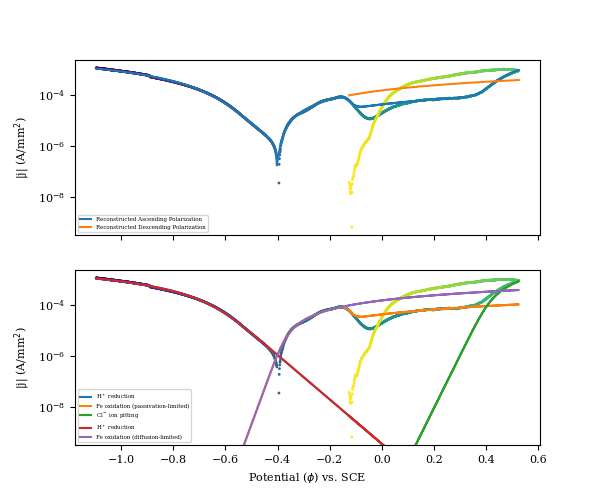
\includegraphics[width=5.0in]{resources/fig_2a2.png}
		\caption{Top: Fitted HCl curves generated by deconvolution procedure.  Bottom: Individual reaction components fitted using Equations \ref{eqn:bv_w} and \ref{eqn:rho_jmak}.}
		\label{fig:hcl_deconv}
	\end{figure}


